\section{Experiment}

We conduct EBARS in the knot inference and manifold denoising. For the knot inference, the performance is compared with the segmented method of \citet{muggeo2003estimating} and the modified maximum likelihood (MML) method of \citet{doi:10.1080/01621459.2021.1947307}. %We calculate the absolute errors of the estimated knots for evaluation. 
For the manifold denoising, the performance is compared with manifold fitting under unbounded noise (MFUN) of \citet{yao2023manifoldfitting}, putative manifold fitting (PMF) of \citet{pmlr-v75-fefferman18a}, principal manifold estimation (PME) of \citet{10.1111/rssb.12416} and principal curves (PC) of \citet{principalcurve}. %We calculate the geometric mean squared distance for evaluation. 
Numerical experiments show that the proposed method performs well in finite samples of all scenarios.

% \subsection{Curve spline regression}

%We conduct EBARS in curve spline regression and compare its prediction performance with BARS method \citep{10.1093/biomet/88.4.1055} and smoothing spline (SS) method \citep{wahba1990spline,green1994nonparametric}. 
The curves and data samples involved are illustrated in the first column of Figure \ref{fig:curve}. It can be seen that data are generated from $4$ different smoothness functions, denoted as Cases $1.1-1.4$ respectively. Cases $1.1$ and $1.2$ are continuous, whereas Cases $1.3$ and $1.4$ are discontinuous with one or multiple breakpoints. The outcome noise is Gaussian with standard deviation $2$, $2$, $4$, $1$. We compare the prediction performance with BARS and SS in curve fitting. To demonstrate the effect of $\gamma$ in EBIC, we implement $3$ versions of EBARS with $\gamma=1,0.5,0$. All methods are evaluated under sample sizes $m=200,500$ and the experiment is repeated $50$ times in each setting.

\begin{figure}
    \centering
    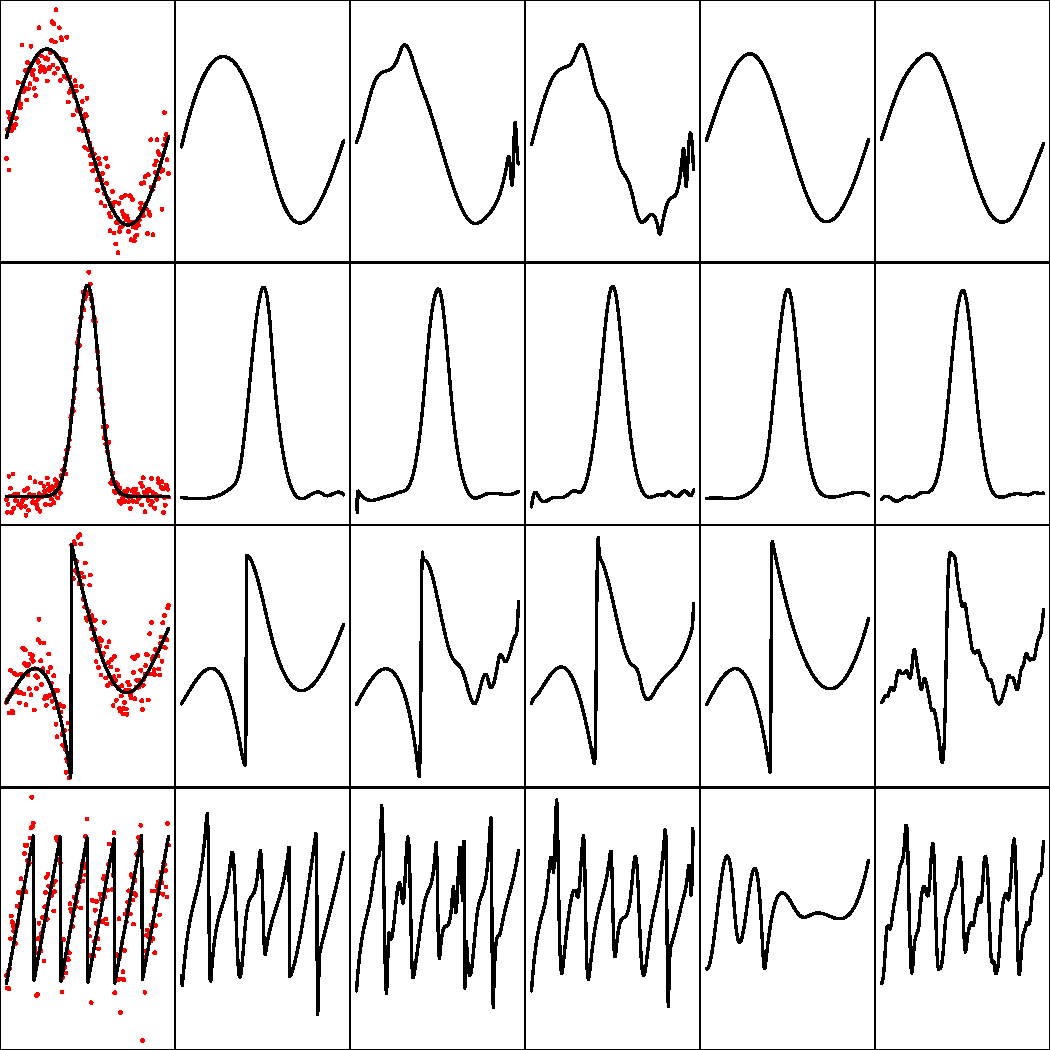
\includegraphics[width=0.85\textwidth]{Experiments/plots/curve_regression.pdf}
    \caption{Curve spline regression. It corresponds to the prediction results with $m=200$ in Cases $1.1-1.4$. From left to right, columns are respectively the ground truth with red observed points, prediction by EBARS with $\gamma=1,0.5,0$, prediction by BARS and prediction by smoothing splines.}
    \label{fig:curve}
\end{figure}

The mean squared errors are summarized in Table \ref{tab:curve}. To remove the effect of outliers, we drop out points with errors in the top or bottom $2.5\%$ to calculate censored MSE on test data. In EBARS, low $\gamma$ causes the model overfitting problem. It is clear that MSE rises up gradually as $\gamma$ decreases, especially in Case $1.3$. The behaviour is visualized in columns $2-4$ of Figure \ref{fig:curve}. This phenomenon is consistent with the theory. According to EBIC, the prior probability of the model space with $k$ knots satisfies $\pi(\mathcal{M}_k)\propto \tau(\mathcal{M}_k)^{1-\gamma}$. As $k<<n$ in practice, $\tau(\mathcal{M}_k)$ will grow with increasing number of knots. Consequently, the lower $\gamma$ means the higher $\pi(\mathcal{M}_k)$ for large $k$. Thereby more knots will be selected into the model, leading to overfitting in the end.

In this example, $\gamma=1$ gives the best performance among EBARS. Furthermore, BARS achieves similar results to EBARS $\gamma=1$ if the true knot number is relatively small, illustrated as in Cases $1.1-1.3$. However, when the required knot number is really large, BARS fails to work completely and attains a terrible MSE. See the $(4,5)$ panel of Figure \ref{fig:curve} for a graphical explanation. Besides, the smoothing spline method has a severe overfitting problem in Case $1.3$, as shown in the $(3,6)$ panel of Figure \ref{fig:curve}. This indicates that splines with many misplaced knots are inferior to adaptive knot splines in discontinuous cases.

\begin{table}
\caption{MSE on test data of five methods in Cases $1.1-1.4$}
\label{tab:curve}
\centering
\begin{tabular}{cccccccc}
\toprule
       Methods     &   $m$  & Case 1.1     & Case 1.2     & Case 1.3     & Case 1.4     \\ \midrule                               
                 
EBARS $\gamma=1$      & \multirow{5}{*}{$200$}     & 0.181(0.124) & 0.332(0.118) & 0.828(0.529) & 0.370(0.366)  \\
EBARS   $\gamma=0.5$  &       & 0.230(0.136)  & 0.389(0.184) & 1.412(0.783) & 0.368(0.150)  \\
EBARS   $\gamma=0$    &     & 0.341(0.229) & 0.464(0.201) & 1.960(0.985)  & 0.418(0.155) \\
BARS       &      & 0.178(0.150)  & 0.368(0.139) & 0.731(0.403) & 3.003(0.504) \\
SS &  & 0.137(0.088) & 0.329(0.132) & 3.772(1.687) & 0.443(0.155) \\
\midrule
EBARS $\gamma=1$     & \multirow{5}{*}{$500$}     & 0.068(0.033) & 0.147(0.061) & 0.361(0.168) & 0.079(0.033) \\
EBARS     $\gamma=0.5$   &    & 0.082(0.039) & 0.156(0.059) & 0.536(0.215) & 0.112(0.034) \\
EBARS    $\gamma=0$   &     & 0.170(0.073)  & 0.231(0.083) & 1.053(0.410)  & 0.144(0.042) \\
BARS        &     & 0.071(0.032) & 0.160(0.054)  & 0.317(0.140)  & 0.364(0.615) \\
SS & & 0.053(0.026) & 0.139(0.041) & 1.914(0.418) & 0.229(0.066) \\
\bottomrule
\end{tabular}
\end{table}
\subsection{Knot inference}

%In many problems, the quantities of main interest are change-points or break-points in the model, such as change-points detection in time series \citep{aminikhanghahi2017survey,truong2020selective}. Thus researchers want to construct an accurate estimation for change-points with rigorous statistical approaches \citep{doi:10.1080/01621459.2015.1073154,doi:10.1080/01621459.2021.1947307}. 
We perform EBARS for knot inference in linear spline regression. % The linear spline is a piecewise linear model. 
Line segments are connected in unique knots and the spline is discontinuous at the location where two knots coincide. The data is generated from three linear spline models with one, two and four knots as shown in Figure \ref{fig:knot_estimation}, where the knot locations are respectively $(0.5),~(0.3,0.7),~(0.2,0.2,0.5,0.7)$. The functions are continuous except for the spline with $k=4$. The noise is Gaussian with standard deviation $0.4$, $0.3$, $0.4$. 

\begin{figure}
    \centering
    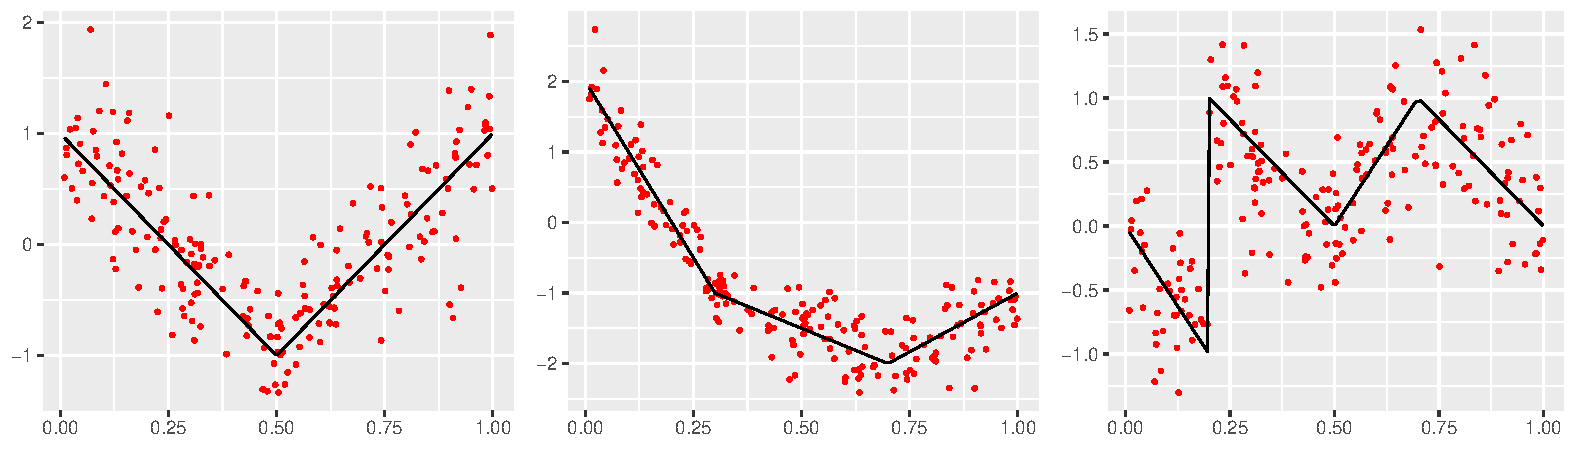
\includegraphics[width=0.9\textwidth]{Experiments/plots/knot_estimation.pdf}
    \caption{Linear splines with one, two and four knots. Black segments are true spline curves and red points are noisy observed data with $m=200$.}
    \label{fig:knot_estimation}
\end{figure}

Figure \ref{fig:knot_inference} illustrates the posterior distribution of the knot number and location by EBARS with $\gamma=1$ in $k=1,2,4$. The sample size is $500$ in all scenarios. We simulate $5000$ samples of $(k,\xi)$ via RJMCMC after $5000$ burning steps. Histograms show that the average knot number is close to the true value with negligible error. From the density plots, the posterior mass concentrates on the correct location of change points in all cases even though the knot number is unknown. Especially, for $k=4$, the posterior density at $0.2$ is double at $0.5$ and $0.7$, meaning that $0.2$ is chosen as the knot twice.

\begin{figure}
    \centering
    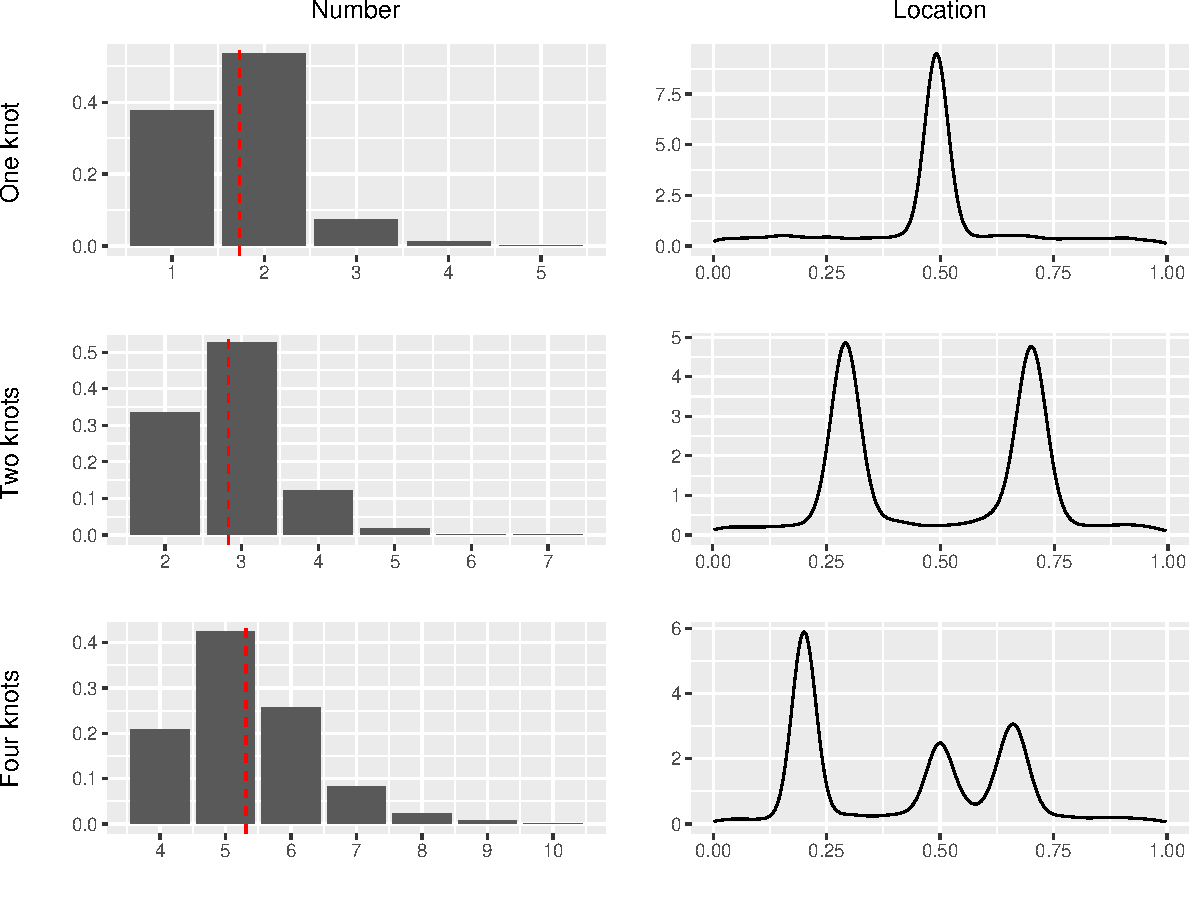
\includegraphics[width=0.9\textwidth]{Experiments/plots/knot_inference.pdf}
    \caption{The posterior distributions of knots in three scenarios by EBARS. Left channels are the histograms of the knot number, where red dashed vertical lines indicate the mean number. Right channels are the posterior density plots of the knot location.}
    \label{fig:knot_inference}
\end{figure}

To evaluate the performance of knot inference, we compare EBARS with Segmented of Muggeo and MML of Guangyu Yang and Zhang. In this experiment, the knot number is given since Segmented and MML cannot estimate $k$. The absolute error of knot location is calculated as criteria. Three methods are evaluated under sample sizes $m=200,500$ and the experiment is repeated $50$ times.

Simulation results of the mean and standard deviation of absolute errors are summarized in Tables \ref{tab:knot_1} and \ref{tab:knot_2}. When $k=1,2$, three methods obtain fairly small absolute errors. However, when $k=4$, the absolute errors of EBARS are much less than other two algorithms for all knots. MML struggles to estimate the duplicate knots $0.2$ and causes horrible bias. Segmented outperforms MML but it is still much less accurate than EBARS. Compared with MML and Segmented, our EBARS is robust and attain a precise estimation with jumping discontinuity and increasing number of knots. Furthermore, MML and Segmented are exclusively applied in linear splines and they require the knot number to be given, whereas EBARS is convenient to estimate the knot number and location simultaneously in splines of any degree.

% In this subsection, we perform EBARS for knot inference in linear spline regression given the knot number $k$. The linear spline is a piecewise linear model. Line segments are connected in unique knots and the spline is discontinuous at the location where two knots coincide. Furthermore, since $k$ is fixed, relocation becomes the only possible movement strategy in MCMC. Consequently, $\gamma$ has no effect on EBARS in this example. We compare its performance with Segmented and MML.
%Notably, their approaches are frequentist whereas EBARS is Bayesian.

% The simulation data are generated from three linear spline population models with one, two and four knots as shown in Figure \ref{fig:knot_estimation}. The knot locations are respectively $(0.5),~(0.3,0.7),~(0.2,0.2,0.5,0.7)$.  %We refer to them as Cases $2.1-2.3$. 

% The functions are continuous except for the spline with $k=4$ at $0.2$. The noise is Gaussian with standard deviation $0.4$, $0.3$, $0.4$. All methods are evaluated under sample sizes $m=200,500$ and the experiment is repeated $50$ times in each setting. Assuming that the $i$-th knot is $\xi_i$ and the estimation is $\hat{\xi}_i$, we calculate the absolute error $|\xi_i-\hat{\xi}_i|$ for each knot. 


% Simulation results are summarized in Tables \ref{tab:knot_1} and \ref{tab:knot_2}. When $k=1,2$, MML and Segmented perform slightly better than EBARS and all three methods obtain fairly small absolute errors. However, when $k=4$, the absolute errors of EBARS are much less than other algorithms for all knots. MML struggles to estimate the duplicate knots $0.2$ and causes horrible errors. Segmented outperforms MML but it is still much less accurate than EBARS. This means that our EBARS is robust and attain a precise estimation with jumping discontinuity and increasing number of knots.

% Furthermore, the MML and segmented methods are exclusively applied in linear spline models. In contrast, EBARS can handle splines of any degree with ease. Moreover, we can estimate the number and locations of knots meanwhile in EBARS, whereas MML and Segmented require $k$ to be given. This is especially important when $k$ is also of interest. Although the computational time of EBARS is relatively longer due to MCMC, EBARS is in favor if speed is not the main concern. 

\begin{table}
\caption{Absolute errors for knot location estimation of three methods in $k=1,2$}
\label{tab:knot_1}
\centering
\begin{tabular}{ccccc}
\toprule
\multirow{2}{*}{Methods} & \multirow{2}{*}{m}   & One knot       & \multicolumn{2}{c}{Two knots}    \\
\cline{3-5}
                         &                      & Knot $1$         & Knot 1         & Knot 2         \\
                         \midrule
EBARS                    & \multirow{3}{*}{200} & 0.0219(0.0126) & 0.0167(0.0150)  & 0.0248(0.0257) \\
MML                      &                      & 0.0163(0.0099) & 0.0138(0.0118) & 0.0170(0.0214)  \\
Segmented                &                      & 0.0159(0.0102) & 0.0117(0.0113) & 0.0186(0.0204) \\
\midrule
EBARS                    & \multirow{3}{*}{500} & 0.0100(0.0076)  & 0.0095(0.0065) & 0.0142(0.0122) \\
MML                      &                      & 0.0075(0.0060)  & 0.0068(0.0058) & 0.0102(0.0076) \\
Segmented                &                      & 0.0079(0.0061) & 0.0070(0.0059)  & 0.0113(0.0081) \\
\bottomrule


\end{tabular}
\end{table}

\begin{table}
\caption{Absolute errors for knot location estimation of three methods in $k=4$}
\label{tab:knot_2}
\centering
\begin{tabular}{cccccc}
\toprule
\multirow{2}{*}{Methods} & \multirow{2}{*}{m}   & \multicolumn{4}{c}{Four knots}                                      \\
\cline{3-6}
                         &                      & Knot 1         & Knot 2         & Knot 3         & Knot 4         \\
                         \midrule
EBARS                    & \multirow{3}{*}{200} & 0.0058(0.0060) & 0.0044(0.0043) & 0.0206(0.0199) & 0.0170(0.0096) \\
MML                      &                      & 0.3437(1.1010) & 0.1163(0.1283) & 0.0978(0.1006) & 0.1012(0.1454) \\
Segmented                &                      & 0.0366(0.0494) & 0.0712(0.1067) & 0.0799(0.0889) & 0.0752(0.0805) \\
\midrule
EBARS                    & \multirow{3}{*}{500} & 0.0025(0.0029) & 0.0026(0.0025) & 0.0194(0.0172) & 0.0150(0.0137) \\
MML                      &                      & 0.2737(0.4266) & 0.1725(0.1683) & 0.1065(0.1800) & 0.2131(0.5211) \\
Segmented                &                      & 0.0171(0.0346) & 0.0283(0.0775) & 0.0395(0.0825) & 0.0349(0.0805) \\
\bottomrule
\end{tabular}
\end{table}
% \subsection{Surface spline regression}

%We utilize tensor product splines to construct EBARS in bivariate spline regression and compare the performance with the BARS method and the thin plate spline (TPS) method of \citet{10.1111/1467-9868.00374}.
We compare the performance with BARS and TPS in the surface fitting.
%TPS is a popular spline-based approach for regression with multidimensional covariates.
The data is generated from four surfaces, denoted as Cases 2.1-2.4. Specifically, Cases 2.1 and 2.2 are smooth, whereas Cases 2.3 and 2.4 are discontinuous. Besides, Case 2.3 is with one jumping point in $x_1$ and Case 2.4 is with two jumping points in $x_1$ and $x_2$ separately. The outcome noise is Gaussian with standard deviation $1,1.5,2,2$. To remove outliers in discontinuous cases, we calculate MSE on test data without the upper or lower $2.5\%$ error. All methods are evaluated under sample sizes $m=500,1000$ and each experiment is repeated $20$ times.

\iffalse
\begin{figure}
    \centering
    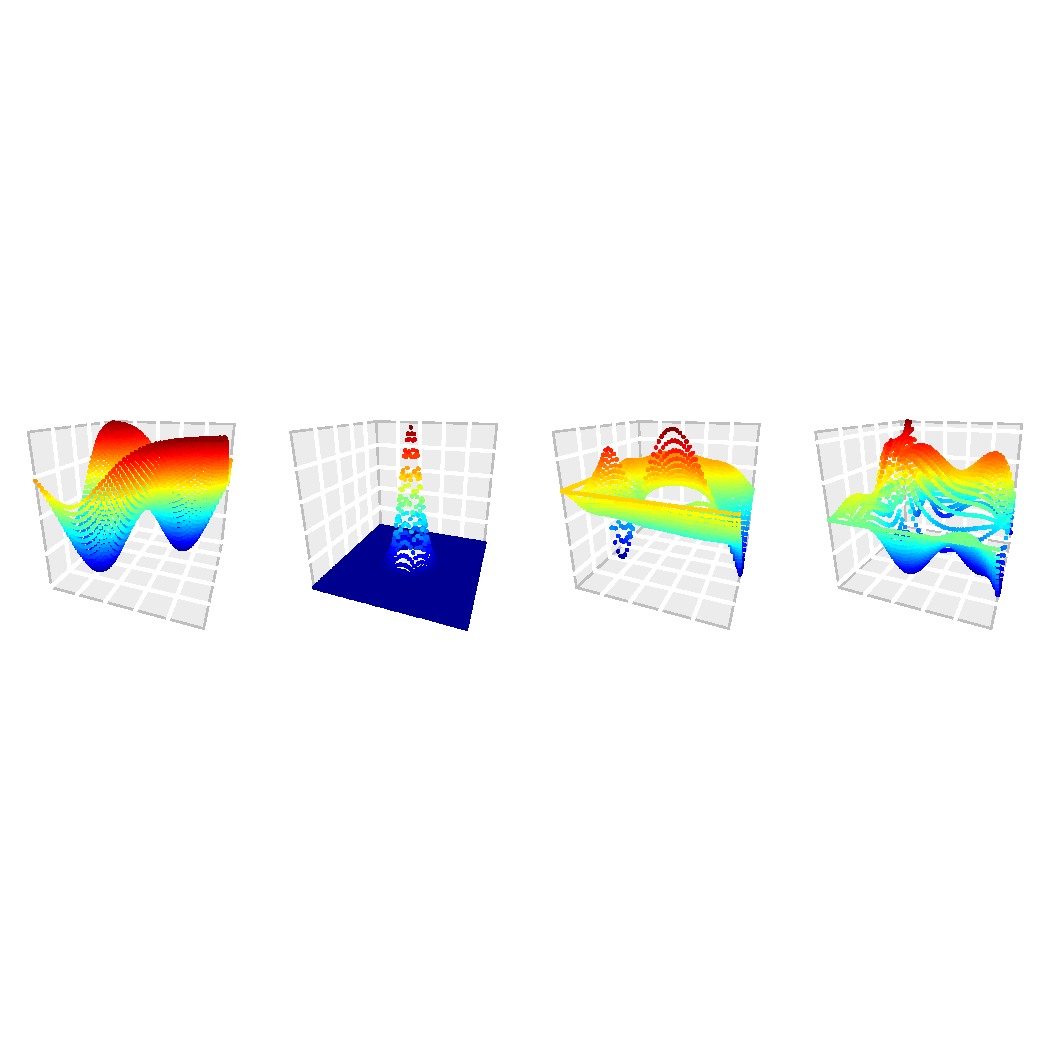
\includegraphics[width=1\textwidth]{Experiments/plots/crop_surface_truth.pdf}
    \caption{The ground truth in surface spline regression for Cases $2.1-2.4$. Cases 2.1 and 2.2 are continuous, whereas Cases 2.3 and 2.4 are discontinuous.}
    \label{fig:surface_truth}
\end{figure}
\fi

The mean squared errors are summarized in Table \ref{tab:surface}. Three EBARS versions with $\gamma=1,0.5,0$ are implemented to demonstrate the effect of $\gamma$. In Cases 2.1 and 2.2, the performance of all five methods is satisfactory and MSE of TPS is roughly the smallest. This indicates that five spline approaches do well in fitting smooth surfaces. However, when the surface is discontinuous, the prediction performance of TPS is worse than free knot splines. For example, the MSE of TPS are much larger than that of EBARS and BARS in Cases 2.3 and 2.4. BARS achieves close results to EBARS except for Case 2.4. As $k$ has to be large enough to fit Case 2.4, the performance of BARS is limited owing to the poor property of BIC in high dimension. Besides, EBARS performs slightly better with low $\gamma$ than with high $\gamma$ even in smooth cases, different from curve regression. It seems that surface regression is more likely to be underfitting rather than overfitting.

\begin{table}
\caption{MSE on test data of five methods in Cases $2.1-2.4$}
\label{tab:surface}
\centering
\begin{tabular}{cccccc}
\toprule
Methods & m                     & Case 2.1     & Case 2.2     & Case 2.3     & Case 2.4     \\
\midrule
EBARS $\gamma=1$   & \multirow{5}{*}{500}  & 0.163(0.044) & 0.624(0.107) & 0.664(0.216) & 1.133(0.443) \\
EBARS $\gamma=0.5$  &                       & 0.148(0.038) & 0.616(0.111) & 0.597(0.192) & 1.101(0.287) \\
EBARS  $\gamma=0$ &                       & 0.138(0.042) & 0.609(0.089) & 0.568(0.136) & 1.076(0.269) \\
BARS    &                       & 0.169(0.050) & 0.671(0.160) & 0.660(0.199) & 1.968(0.485) \\
TPS     &                       & 0.102(0.031) & 0.587(0.092) & 1.958(0.625) & 2.324(0.466) \\
\midrule
EBARS $\gamma=1$  & \multirow{5}{*}{1000} & 0.064(0.011) & 0.355(0.051) & 0.230(0.061) & 0.331(0.077) \\
EBARS $\gamma=0.5$  &                       & 0.066(0.016) & 0.326(0.056) & 0.222(0.053) & 0.343(0.078) \\
EBARS $\gamma=0$  &                       & 0.065(0.014) & 0.306(0.058) & 0.242(0.067) & 0.336(0.058) \\
BARS    &                       & 0.107(0.027) & 0.416(0.094) & 0.313(0.074) & 1.020(0.510) \\
TPS     &                       & 0.057(0.015) & 0.319(0.032) & 1.205(0.215) & 1.379(0.214) \\
\bottomrule
\end{tabular}
\end{table}

To graphically illustrate the difference in surface spline regression, we visualize the prediction results with $m=1000$ by contour maps in Figure \ref{fig:surface}. Initially, the fitted contours approximately overlap with the ground truth in Cases 2.1 and 2.2, see the top $2$ rows. We can see from the $(3,6)$ and $(4,6)$ panels that TPS fails to estimate the jump discontinuity in Cases 2.3 and 2.4. Actually, the fitted surfaces by TPS are always smooth regardless of the smoothness of true models. BARS obtains a nice performance in Cases 2.1-2.3, but is trapped in Case 2.4 when the required $k$ is enormous. Conversely, Columns $2-4$  of Figure \ref{fig:surface} show that our EBARS makes precise predictions in all cases successfully.

\begin{figure}
    \centering
    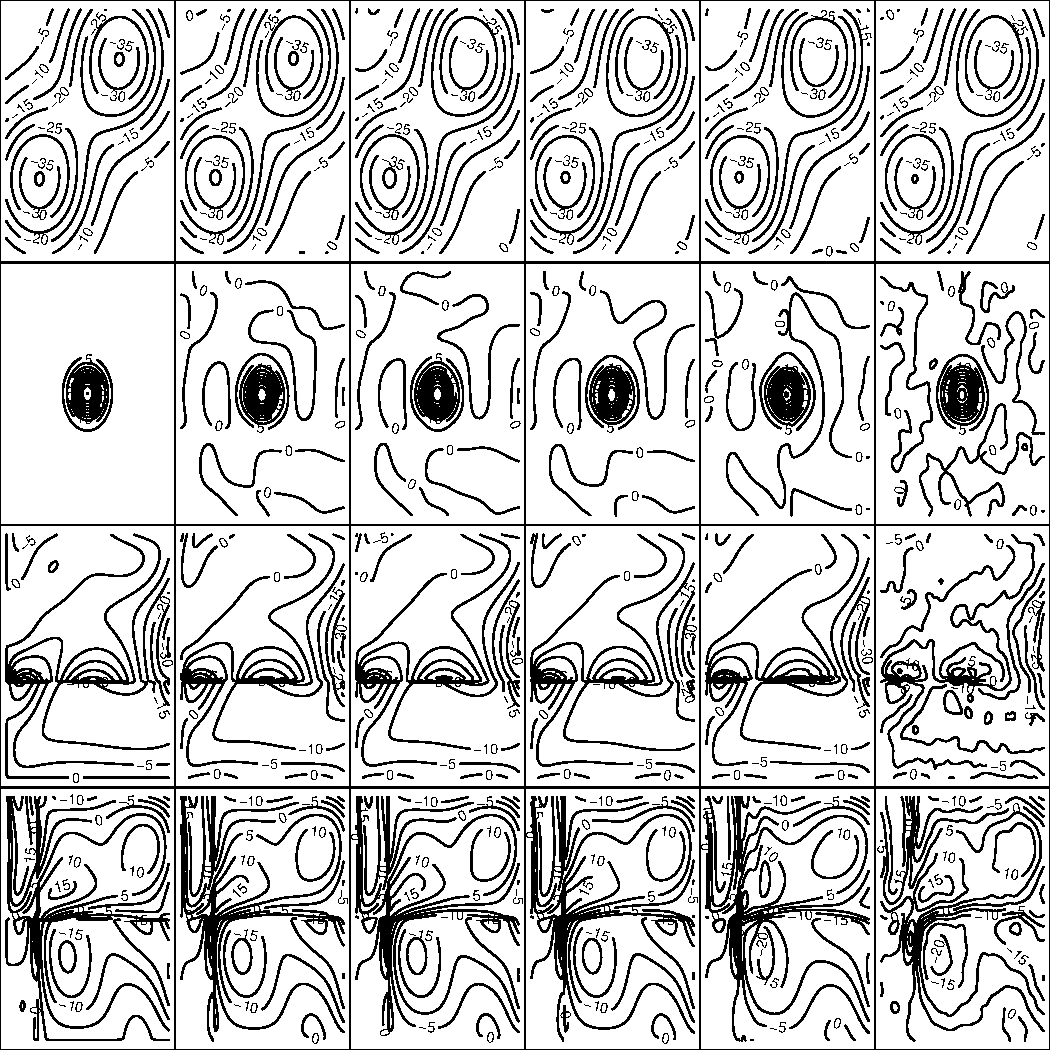
\includegraphics[width=0.85\textwidth]{Experiments/plots/surface_regression.pdf}
    \caption{Surface spline regression. It illustrates the prediction results with $m=1000$ in Cases $2.1-2.4$ by contours. From left to right, columns are respectively the ground truth, prediction by EBARS with $\gamma=1,0.5,0$, prediction by BARS and prediction by TPS.}
    \label{fig:surface}
\end{figure}

%\section{Application}
\subsection{Manifold denoising}

With the assumption of linearity, principal component analysis is a prevailing and efficient method for dimension reduction in high-dimensional space. However, the simple method poses a limitation to respect the nonlinear relationship. 
% Thus, it is essential to develop a powerful and sophisticated approach for nonlinear data analysis. 
Manifold estimation is a technique for modelling the complicated dependence in high-dimensional data, denoising the observations and estimating the low-dimensional latent manifold. Refer to \citet{doi:10.1073/pnas.2311436121} for a detailed review about manifold estimation. 
%Many statistical models have been established to achieve the objective, such as CycleGAN of \citet{doi:10.1073/pnas.2311436121} and principal manifold estimation (PME) of \citet{10.1111/rssb.12416}.

Assume that the observed data $\{x_i\}_{i=1}^m$ is generated from a low-dimensional latent manifold of a high-dimensional ambient space with random noise. That is,
\begin{equation*}
    X=W+\epsilon, \quad X,\epsilon\in \mathbb{R}^D,~W\in \mathbb{M}^d,
\end{equation*}
where $\mathbb{M}^d$ is a $d$-dimensional submanifold of $\mathbb{R}^D$ with $d\leq D$, $W$ is generated from a probability distribution supported in $\mathbb{M}^d$, and $\epsilon$ is $D$-dimensional noise independent of $W$. %The main objective of the manifold estimation is to fit the latent manifold by using $\{x_i\}_{i=1}^m$. According to differentiable geometry, a $d$-dimensional Riemannian manifold with global parametrization is determined by an exponential map $f=(f_1,\ldots,f_D):\mathbb{R}^d\rightarrow \mathbb{M}^d\subset \mathbb{R}^D$, where $\mathbb{R}^d$ is the corresponding tangent space. Therefore, the manifold estimation is also equivalent to finding such a parametrization.
In this article, we propose a two stage manifold estimation (TSME) technique for modelling $\mathbb{M}^d$. The primary challenge of parametrization is attributed to the lack of the required pairs of training data, \emph{i.e.}, (predictor, response). %Thus, it is an unsupervised learning problem. 
We resolve the issue simply by combining the manifold embedding and reconstruction. The manifold embedding is a nonlinear dimensional reduction method. Many impressive algorithms have been proposed in the literature, such as ISOMAP \citep{balasubramanian2002isomap}, Laplacian eigenmaps \citep{belkin2003laplacian} and UMAP \citep{mcinnes2018umap}. 

At the first stage, we apply the manifold embedding technique in $\{x_i\}_{i=1}^m$ given the intrinsic dimension $d$, yielding a projection map $\hat{g}:\mathbb{R}^D\rightarrow \mathbb{R}^d$. Let $u_i=\hat{g}(x_i)$ for $i=1,\ldots,m$. Then $\{(u_i,x_i)\}_{i=1}^m$ are the training samples for the manifold reconstruction. At the second stage, we execute the regression in $\{(u_i,x_i)\}_{i=1}^m$ to reconstruct the manifold. For example, we can use the proposed EBARS method to estimate the reconstruction map $\hat{f}$. Due to the automatic knot selection, EBARS is eligible to model the complex relationships between $u$ and $x$. Consequently, the manifold estimation is completed by the composition of the embedding $\hat{g}$ and the reconstruction $\hat{f}$. Especially, $\{\hat{f}\circ \hat{g}(x_i)\}_{i=1}^m$ can serve as the denoised representation of $\{x_i\}_{i=1}^m$. %Furthermore, the composition $\hat{f}\circ\hat{g}$ can be considered as a solution to the minimum problem of the loss function $\mathbb{E}\left|\left| X-f\circ g(X) \right|\right|^2$.

We conduct the TSME method in manifold denoising and compare its performance with MFUN, PMF, PME and PC. Notably, PME and PC adopt a similar framework with our TSME except that they utilize smoothing splines for reconstruction. The data is generated from two disconnected arcs in $\mathbb{R}^2$, a spiral curve in $\mathbb{R}^2$ and a Swiss roll in $\mathbb{R}^3$, as shown in Figures \ref{fig:d1} and \ref{fig:d2}.%corresponding to $(d=1,D=2)$ and $(d=2,D=3)$. 
ISOMAP is used as the embedding map of TSME and the initial projection of PME in the spiral and  Swiss roll. For the arc case, we substitute UMAP for ISOMAP due to the disconnectivity. Besides, for the Swiss roll, we only compare TSME, MFUN and PMF, as PC is limited to the curve case and PME is very slow with disastrous performance. The random noise is Gaussian with standard deviation $0.2,0.2,1.5$.

Simulation results including the training samples and the denoised data are visualized in Figures \ref{fig:d1} and \ref{fig:d2}. The sample sizes are $m=1000,1500,3000$. Compared with TSME, the PME and PC methods collapse dramatically in curve cases. In arcs, the disconnectivity of $\mathbb{M}^d$ causes the jumping discontinuity of the reconstruction map. %As mentioned above, EBARS is superior to the smoothing splines in describing sharp changes. 
In spiral, the dependency is complex due to the intricate manifold, posing a critical challenge in selecting the optimal penalty weight of smoothing splines. %And the smoothness in EBARS is controlled based on the number of knots without the penalty term. 
For MFUN and PMF, the denoised representations remain corrupted in the spiral and Swiss roll cases. They don't mitigate the random noise successfully and fail to estimate the latent manifolds accurately.

\begin{figure}
    \centering
    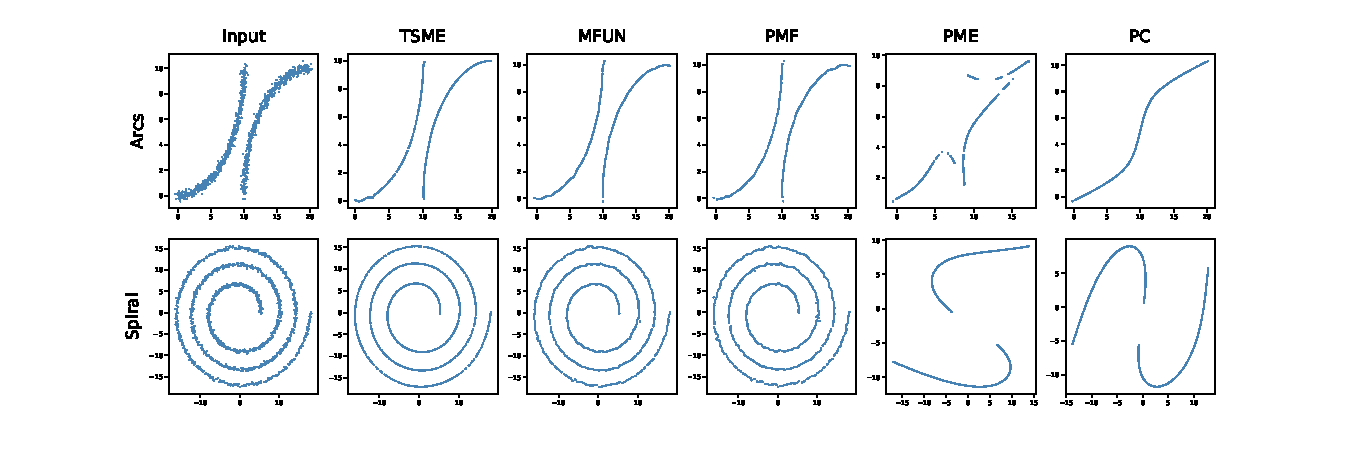
\includegraphics[width=0.9\textwidth]{Experiments/plots/crop_dim1.pdf}
    \caption{Manifold denoise results for two curve scenarios. Each plot indicates the training samples or the denoised representation obtained by our TSME, MFUN, PMF, PME and PC.}
    \label{fig:d1}
\end{figure}

\begin{figure}
    \centering
    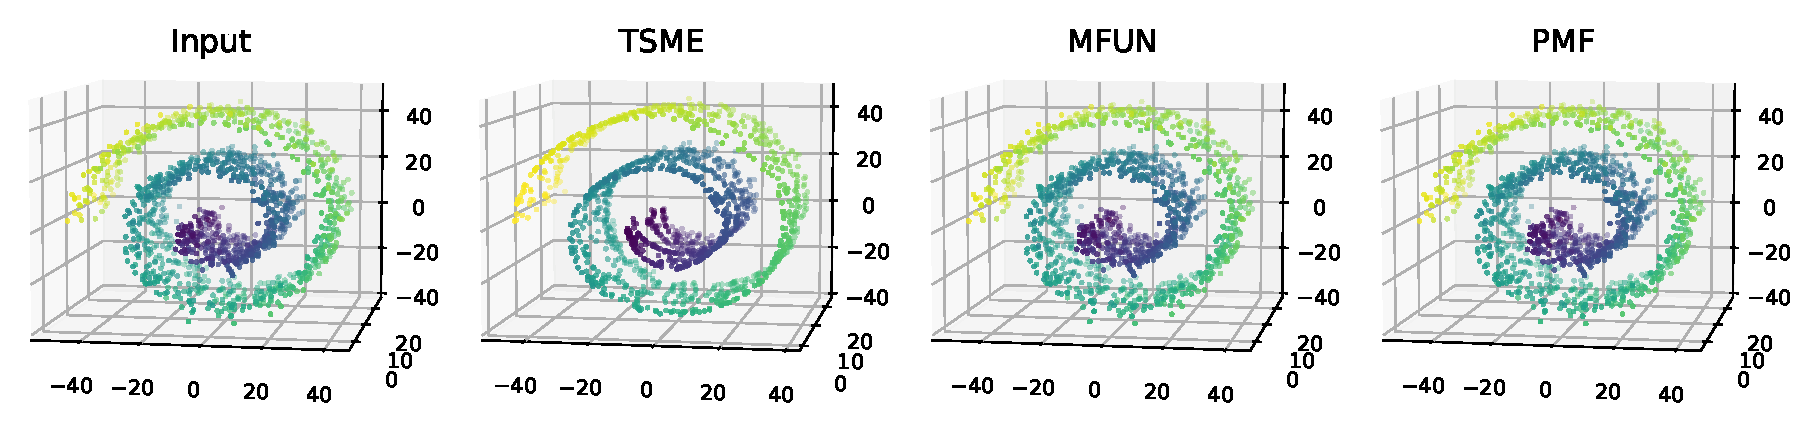
\includegraphics[width=0.95\textwidth]{Experiments/plots/dim2.pdf}
    \caption{Manifold denoise results for the Swiss roll. Each plot indicates the training samples or the denoised representation obtained by our TSME, MFUN and PMF.}
    \label{fig:d2}
\end{figure}

To evaluate the performance quantitatively, we define the geometric mean squared distance as
\begin{equation*}
    \text{GMSD}=\frac{1}{m}\sum_{i=1}^m \text{dist}(\hat{f}\circ\hat{g}(x_i),\mathbb{M}^d)^2,
\end{equation*}
where $\text{dist}(x,\mathbb{M}^d)=\inf_{x'\in\mathbb{M}^d}||x-x'||$. The GMSD measures the corrupted extent of the data away from the manifold. Table \ref{tab:gmsd} illustrates the mean and standard deviation of GMSD in three manifolds of $20$ duplicates. TSME obtains significantly smaller GMSD than the training samples in all scenarios and achieves the smallest GMSD in most cases, demonstrating that our method contributes to excellent manifold denoising. For MFUN and PMF, the performance in the $d=1$ cases is satisfactory but the noise is not reduced in the Swiss roll. PME and PC are completely incapable of estimating the latent manifolds. %This indicates again the great advantage of EBARS over the smoothing spline with equally-spaced fixed knots.

\begin{table}
    \centering
    \caption{Summary of GMSD with respect to five methods in three manifolds}
    \label{tab:gmsd}
    \begin{tabular}{@{}cccc@{}}
    \toprule
          & Arcs                    & Spiral                  & Swiss roll              \\ \midrule
    $m$ & 500 & 1000 & 1500 \\
    Input & 0.0404(0.0020)          & 0.0397(0.0021)          & 2.6033(0.0729)          \\
    TSME  & 0.0036(0.0021)          & 0.0019(0.0003) & 0.5299(0.0653) \\
    MFUN  & 0.0039(0.0011) & 0.0112(0.0011)          & 2.5549(0.0735)          \\
    PMF   & 0.0051(0.0011)          & 0.0165(0.0017)          & 2.5994(0.0733)          \\
    PME   & 0.4790(0.2585)          & 2618.6(9887.4)          &            $\times$             \\
    PC    & 0.7661(0.0077)          & 2.9539(0.0633)          &            $\times$             \\ \midrule
        $m$ & 1000 & 1500 & 3000 \\
    Input & 0.0399(0.0013)          & 0.0401(0.0013)          & 2.6423(0.0621)          \\
    TSME  & 0.0044(0.0033)          & 0.0015(0.0002) & 0.5004(0.0605) \\
    MFUN  & 0.0018(0.0004) & 0.0078(0.0005)          & 2.5377(0.0629)          \\
    PMF   & 0.0023(0.0007)          & 0.0113(0.0008)          & 2.6241(0.0625)          \\
    PME   & 0.3135(0.1353)          & 151.87(449.52)          &            $\times$             \\
    PC    & 0.7589(0.0072)          & 2.9601(0.0699)          &            $\times$             \\ 
    \bottomrule
\end{tabular}
\end{table}


\iffalse
The so-called principal manifold is the minimizer of the following objective function in a well-defined functional space,
\begin{equation}
\label{eq:pme}
    \mathbb{E}\left|\left| X-f(\pi_f(X)) \right|\right|^2 + \lambda \sum_{l=1}^D \int_{\mathbb{R}^d} \sum_{i,j=1}^d \left|\frac{\partial^2 f_l}{\partial t_i \partial t_j}(t)\right|^2 dt,
\end{equation}
where $\lambda$ is the penalty weight, $f:\mathbb{R}^d\rightarrow \mathbb{M}^d \subset \mathbb{R}^D$ is equivalent to the exponential map and $\pi_f:\mathbb{R}^D\rightarrow \mathbb{R}^d$ is the corresponding projection. The PME algorithm solves \eqref{eq:pme} in an iterative fashion. That is, given an initial estimation, $f_{n+1}=\arg \min  \mathbb{E}\left|\left| X-f(\pi_{f_n}(X)) \right|\right|^2 + \text{penalty}$. \citet{10.1111/rssb.12416} utilizes thin plate splines to compute $f_{n}$ with $\pi_{f_0}$ given by ISOMAP \citep{balasubramanian2002isomap}. In this example, we substitute EBARS for thin plate splines to estimate manifolds and compare their performance. In addition, the practice suggests that more iteration steps have little effect on the improvement. Thereby we just update one step. Consequently, the overall manifold fitting algorithm is to solve the least-square problem $\frac{1}{m}\sum_{i=1}^m ||x_i-f(\pi_{f_0}(x_i))||^2$, where $\{x_i\}_{i=1}^m\subset \mathbb{R}^D$ are data samples and $f$ is estimated by EBARS.

The data involved is illustrated in Column 1 of Figure \ref{fig:manifold_fitting}. It consists of the spiral curve in $\mathbb{R}^2$, the space spiral in $\mathbb{R}^3$ and the Swiss roll in $\mathbb{R}^3$, corresponding to $(d=1,D=2)$, $(d=1,D=3)$ and $(d=2,D=3)$ respectively. The noise is Gaussian with standard deviation $0.35,0.4,0.5$. The sample sizes for the three cases are $1000,1000,2000$. The estimated manifolds are visualized in Columns 2 and 3 of Figure \ref{fig:manifold_fitting}. The PME method collapses dramatically due to the complex intrinsic structures, leading to meaningless manifolds as shown in Column 3. On the contrary, it is surprising to find that the EBARS method fits excellent latent manifolds in three cases as shown in Column 2. The primary reason is that the optimal choice of $\lambda$ in \eqref{eq:pme} causes a challenge for the PME algorithm, whereas it doesn't involves any penalty in EBARS. The impressive results again indicate great advantages of EBARS over equally-spaced knot splines.


\begin{figure}[ht]
    \centering
    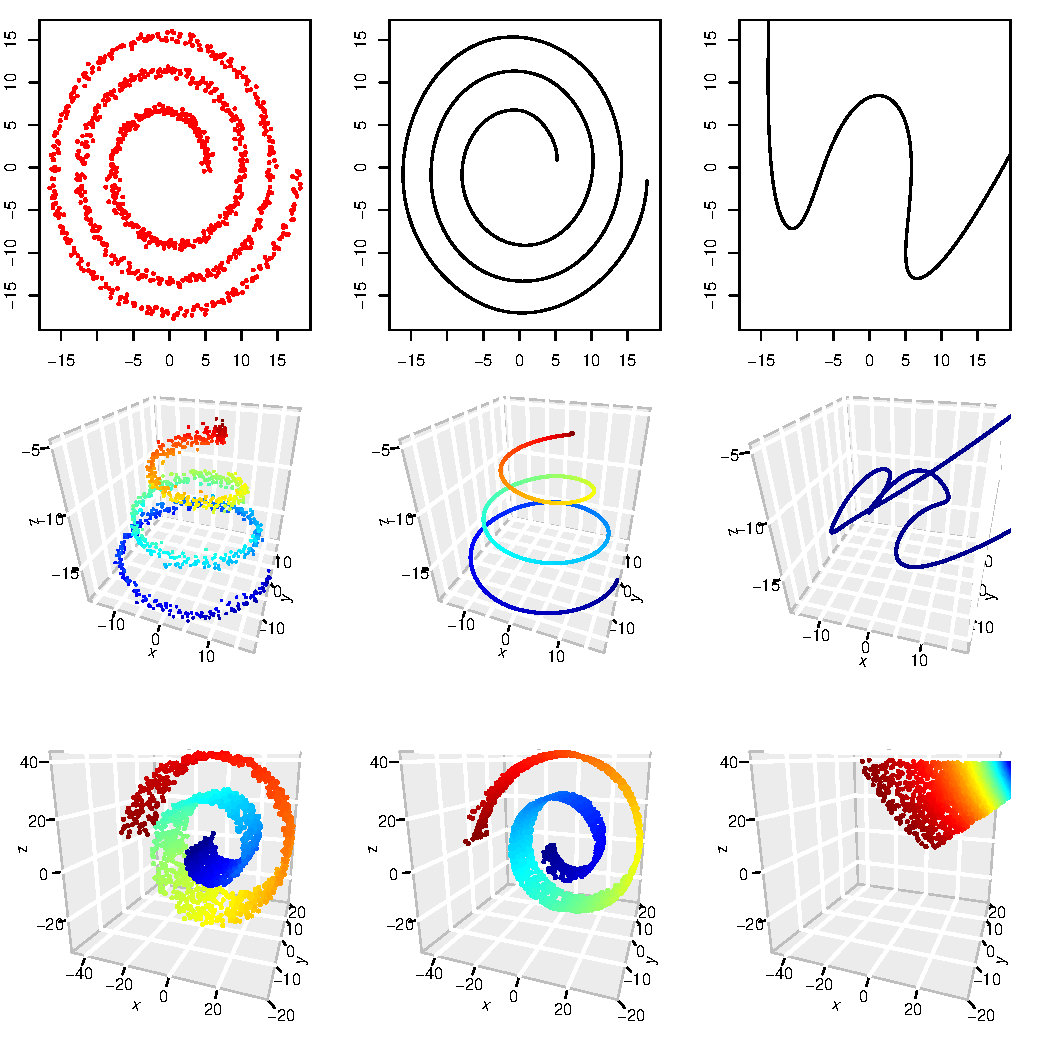
\includegraphics[width=1\textwidth]{Experiments/plots/manifold_fitting.pdf}
    \caption{Manifold fitting for spiral curves in $\mathbb{R}^2$ and $\mathbb{R}^3$ and Swiss roll in $\mathbb{R}^3$. Column 1: the ground truth. Column 2: fitting by EBARS. Column 3: fitting by PME.}
    \label{fig:manifold_fitting}
\end{figure}
\fi
%\subsection{Real data analysis}

We will add a real data example in the future. It may be related to the brain surface fitting of HCP fMRI, or change-point detection in time series. We prefer HCP data if the performance is impressive.